%%%%%%%%%%%%%%%%%%%%%%%%%%%%%%%%%%%%%%%%%%%%%%%%%%%%%%%%%%%%%%%%%%%%%%
% Lớp 10 | Hàm số bậc hai và đồ thị | Hàm số bậc hai
% Dạng 0D3?2-3: Đồ thị của hàm số bậc hai
% Số câu: 40  (sinh tự động bởi tach_cau.py; từ nay thầy sửa trực tiếp file này)
%%%%%%%%%%%%%%%%%%%%%%%%%%%%%%%%%%%%%%%%%%%%%%%%%%%%%%%%%%%%%%%%%%%%%%

%%%%%%%%%%%%%%%% TRẮC NGHIỆM 4 PHƯƠNG ÁN %%%%%%%%%%%%%%%%

% nguồn: MaHoaNH_TracNghiem_Lop10
\begin{ex}%[0D3N2-3]%[ma:c7d0f4d4]
	Đồ thị hàm số $y=x^2-2  x-3$ đi qua điểm nào sau đây?
	\choice 
		 {$N(1; 2)$ }
		{$P(0; 2)$} 
		{$M(1;  1)$ }
		{\True $Q(3;  0)$}
	\loigiai{ 
	Đồ thị  hàm số đi qua điểm $Q(3; 0)$, vì khi thay $x=3$ ta có $y=3^2-2 \cdot 0-3=0$.}
\end{ex}

% nguồn: MaHoaNH_TracNghiem_Lop10
\begin{ex}%[0D3N2-3]%[ma:34157212]
	Trục đối xứng của Parabol $(P)\colon y=2x^2+6x+3$ là đường thẳng nào sau đây? 
	\choice 
		 {$x=\dfrac{3}{2} $}
		 {$y=\dfrac{3}{2} $}
		 {$y=-\dfrac{3}{2} $}
		 {\True $x=-\dfrac{3}{2} $}
	\loigiai{ 
		Trục đối xứng của Parabol  là $x=-\dfrac{b}{2a}=-\dfrac{3}{2}$.
	 }
\end{ex}

% nguồn: MaHoaNH_TracNghiem_Lop10
\begin{ex}%[0D3N2-3]%[ma:4f4cac35]
	Cho hàm số bậc hai $y=ax^2+bx+c$  ($a \neq 0$) có đồ thị $(P)$, đỉnh của $(P)$ được xác định bởi công thức nào?
	 \choice
		{$I\left(-\dfrac{b}{a}; -\dfrac{\Delta}{4a}\right)$} 
		{$I\left(\dfrac{b}{2a}; \dfrac{\Delta}{4a}\right)$} 
		{$I\left(-\dfrac{b}{2a};  \dfrac{\Delta}{4a}\right)$}
		{\True $I\left(-\dfrac{b}{2a};-\dfrac{\Delta}{4a}\right)$} 
	\loigiai{ 
		Ta có đỉnh của $(P)$ là $I\left(-\dfrac{b}{2a};  -\dfrac{\Delta}{4a}\right)$.
	 }
\end{ex}

% nguồn: MaHoaNH_TracNghiem_Lop10
\begin{ex}%[0D3N2-3]%[ma:8067846b]
	\immini[thm]{Cho hàm số bậc hai $y=f(x)$ có đồ thị như  hình vẽ. Tập nghiệm của bất phương trình $f(x)>0$ là
	 \choice
		 {$(0;3)$}
		 {$[-1;3]$}
		 {$(-\infty;-1)\cup(3;+\infty)$}
		 {\True $(-1;3)$}
		}{ 
		\begin{tikzpicture}[line join=round,line cap=round,font=\footnotesize,scale=0.6,>=stealth]
				 \draw[-stealth](-1.5,0)--(4,0) node[above]{$x$};
				 \draw[-stealth](0,-2)--(0,4.5) node[right]{$y$};
				\draw[smooth,samples=100,domain=-1.3:3.3] plot (\x,{-(\x+1)*(\x-3)}); 
				\fill (0,0) circle (1pt) node[below  left]{$O$};
				\foreach \x/\g  in {-1/140,3/50}\fill[black] (\x,0) circle (1pt)+(\g:.4) node{$\x$};
			\end{tikzpicture}
		} 
	 \loigiai{
		Nhìn đồ thị ta thấy phần đồ thị nằm trên trục hoành $f(x)>0$  khi $x\in(-1;3)$.
	 }
\end{ex}

% nguồn: MaHoaNH_TracNghiem_Lop10
\begin{ex}%[0D3N2-3]%[ma:3d2e8b24]
	\immini{Cho  đồ thị hàm số sau.
	Điểm thuộc đồ thị hàm  số mà có hoành độ bằng $2$ là
	 \choice
		{$(2;0)$} 
		{\True $(2;3)$} 
		{$(3;2)$} 
		{$(2;-3)$}}{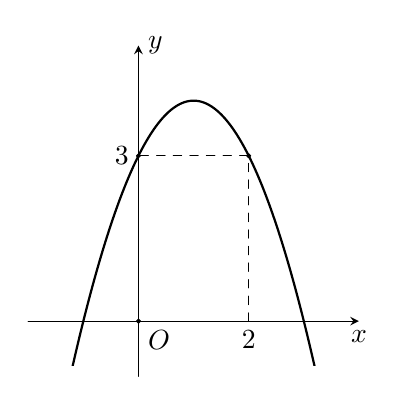
\begin{tikzpicture}[scale=0.7,>=stealth,line join=round,line cap=round,smooth,samples=450,declare function={xmin=-2; xmax=4; ymin=-1; ymax=5;}]
		 \path (0,0) node[below right]{$O$}
			(0,3) node[left]{$3$} 
			(2,0) node[below]{$2$}; 
		 \draw[->] (xmin,0)--(xmax,0) node[below]{$x$};
		 \draw[->] (0,ymin)--(0,ymax) node[right]{$y$};
		\clip  (xmin+.2,ymin+.2) rectangle (xmax-.2,ymax-.2);
		\draw[domain=xmin:xmax,smooth,thick,variable=\x,black] plot ({\x},{-\x*\x + 2*\x  + 3});
		\draw[dashed] (2,0) -- (2,3) --  (0,3);
		 \path[fill=black,draw] (0,3) circle (1pt);
		\path[fill=black,draw] (2,3) circle  (1pt);
		\path[fill=black,draw] (0,0)  circle (1pt);
	\end{tikzpicture}
		} 
	\loigiai{Dựa vào đồ thị ta thấy điểm thuộc đồ thị hàm số có hoành độ bằng $2$ là điểm  $(2;3)$.}
\end{ex}

% nguồn: MaHoaNH_TracNghiem_Lop10
\begin{ex}%[0D3H2-3]%[ma:ea59f432]
	Parabol $y=2x^2-4x+3$ có trục đối xứng là đường thẳng có phương trình là 
	\choice 
		 {$x=2$}
		 {\True $x=1$}
		{$x=-2$} 
		{$x=-1$} 
	 \loigiai{
		Ta có $a=2$, $b=-4$, parabol có trục đối xứng là đường thẳng có phương trình $x=-\dfrac{b}{2a}=1$. 
	 }
\end{ex}

% nguồn: MaHoaNH_TracNghiem_Lop10
\begin{ex}%[0D3H2-3]%[ma:84aaa387]
	\immini[thm]{Cho hình vẽ bên,  biết $f(x)=ax^{2}+bx+c$ và $\Delta=b^{2}-4ac$. Khẳng định nào sau đây đúng?
	\choicew{0.4\textwidth} 
	\choice 
		{$a>0$, $\Delta<0$} 
		{$a<0$, $\Delta<0$} 
		{\True $a>0$,  $\Delta>0$}
		{$a<0$, $\Delta>0$}}{ 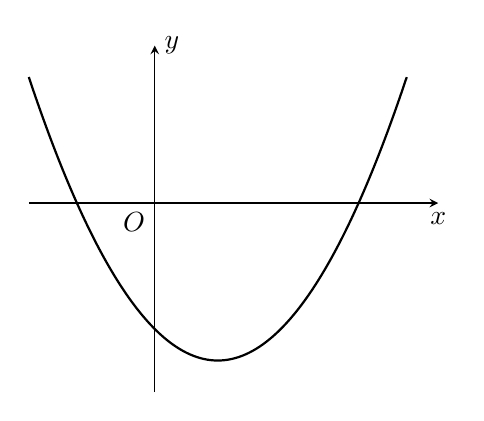
\begin{tikzpicture}[smooth,samples=300,scale=0.8,>=stealth]
		\draw[->] (-2,0)--(4.5,0) node[below]{$x$}; 
		\draw[->] (0,-3)--(0,2.5)  node[right]{$y$};
		\draw (0,0) node[below  left]{$O$};
		\draw[thick,black,domain=-2:4] plot  (\x,{1/2*(\x)^2-(\x)-2});
	\end{tikzpicture}
		 }
	\loigiai{ 
		Đồ thị hàm  số có bề lõm hướng lên nên $a>0$, đồ thị hàm số cắt trục $Ox$ tại $2$ điểm nên $\Delta > 0$.
	 }
\end{ex}

% nguồn: MaHoaNH_TracNghiem_Lop10
\begin{ex}%[0D3H2-3]%[ma:f367b437]
	\immini[thm]{ 
	Hàm số nào có đồ  thị như hình vẽ bên dưới?
	\choice 
		 {\True $y=-x^2+4x-3$}
		{$y=-x^2-4x-3$} 
		 {$y=-2x^2-x-3$}
		{$y=x^2-4x-3$} 
		 }{
		\begin{tikzpicture}[>=stealth,x=1.0cm,y=1.0cm,scale=0.8]
				\draw[->] (-1,0) -- (4,0) node[below] {\scriptsize  $x$};
				\draw[->] (0,-2.5) --  (0,2) node[right] {\scriptsize $y$};
				\draw[dashed,thin]  (0,1)--(2,1)--(2,0);
				 \draw (0,1) node[left]{\scriptsize $1$}
					(0,0)  node[below left]{\scriptsize O}
					 (2,0) node[below]{\scriptsize $2$};
				\draw[domain=0.2:3.8,samples=150] plot  (\x,{-(\x)^2+4*(\x)-3});
			\end{tikzpicture}
		} 
	 \loigiai{
		Đồ thị có  bề lõm quay xuống dưới nên $a<0$. Trục đối xứng $x=2$.\\
		Vậy đồ thị đã cho là đồ thị hàm số $y=-x^2+4x-3$. 
	 }
\end{ex}

% nguồn: MaHoaNH_TracNghiem_Lop10
\begin{ex}%[0D3H2-3]%[ma:195a4e58]
	\immini[thm]{Cho hàm số $y=a{x^2}+bx+c$ có đồ thị như bên. 
	 Khẳng định nào dưới đây là đúng?
	\choice 
		 {$a > 0,b > 0,c < 0$}
		{$a < 0,b < 0,c  > 0$}
		{$a > 0,b < 0,c >  0$}
		{\True $a > 0,b < 0,c  < 0$}
		}{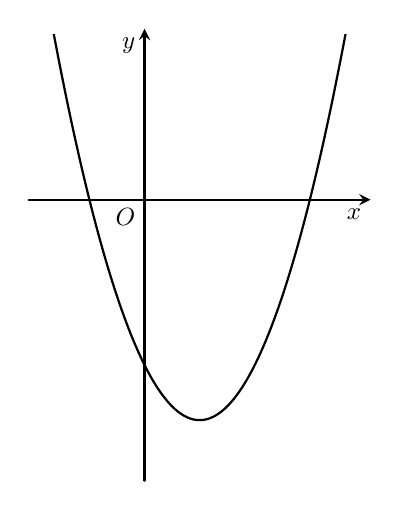
\begin{tikzpicture}[line join=round,line cap=round,>=stealth,thick,scale=0.7]
		\tikzset{every node/.style={scale=0.9}} 
		\draw[->]  (-2.1,0)--(4.1,0) node[below left] {$x$};
		 \draw[->] (0,-5.1)--(0,3.1) node[below left] {$y$};
		\draw  (0,0) node [below left] {$O$};
		\begin{scope}
			\clip  (-2,-5) rectangle (4,3);
			\draw[samples=200,domain=-2:4,smooth,variable=\x]  plot (\x,{1*(\x)^2+-2*(\x)+-3});
		\end{scope}
	\end{tikzpicture}
		} 
	\loigiai{ 
		Đồ thị  cắt trục tung tại điểm có tung độ âm nên $c < 0$.\\
		Đồ thị hướng bề lõm lên trên nên $a > 0$, hoành  độ đỉnh dương nên $\dfrac{-b}{2a}> 0, \,a > 0\Rightarrow b < 0$.
	} 
\end{ex}

% nguồn: MaHoaNH_TracNghiem_Lop10
\begin{ex}%[0D3H2-3]%[ma:90fe15f4]
	\immini{ 
	Cho hàm số $y=f(x)=a x^2+b x+c$  có đồ thị như hình vẽ. Đặt $\Delta=b^2-4ac$, tìm dấu của $a$ và $\Delta$.}
	{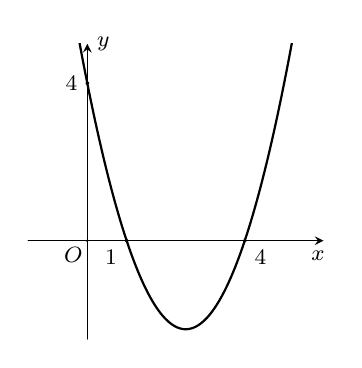
\begin{tikzpicture}[scale=0.5,font=\footnotesize,line join=round,
			line cap=round,>=stealth] 
		\def \xmin{-1.5} 
		\def  \xmax{6}
		\def  \ymin{-2.5}
		 \def \ymax{5}
		\draw[->] (\xmin,0)--(\xmax,0) node[shift=(-110:0.2)]  {$x$};
		\draw[->] (0,\ymin)--(0,\ymax)  node[right] {$y$};
		\fill  (0,0) circle (1pt) node[shift=(-135:0.25)]{$O$};
		\clip (\xmin,\ymin) rectangle (\xmax,\ymax); 
		\draw[smooth,samples=100,domain=\xmin:\xmax,thick] plot (\x,{(\x)^2-5*(\x)+4}); 
		 \foreach \x/\nx in {1/1}
		\draw (\x,0) circle (1pt) node[below left] {$\nx$}; 
		\foreach  \x/\nx in {4/4}
		\draw (\x,0) circle  (1pt) node[below right] {$\nx$};
		\foreach \y/\ny in {4/4} 
		\draw  (0,\y) circle (1pt) node[left] {$\ny$};
	\end{tikzpicture}
	} 
	\choice 
		{\True  $a>0$, $\Delta>0$}
		{$a<0$,  $\Delta>0$}
		{$a>0$, $\Delta=0$} 
		{$a<0$,  $\Delta=0$}
	\loigiai{ 
		Đồ thị hàm số là một parabol có bề lõm quay lên nên $a>0$ và đồ thị hàm số cắt trục $Ox$ tại hai điểm phân  biệt nên $\Delta>0$.
	} 
\end{ex}

% nguồn: MaHoaNH_TracNghiem_Lop10
\begin{ex}%[0D3H2-3]%[ma:0b994c0e]
	\immini[thm]{Đồ  thị hình bên dưới là đồ thị của hàm số nào?
	\choice 
		{$y=2x^2-4x-2$} 
		 {$y=-x^2-2x+3$}
		 {\True$y=x^2-2x-1$}
		 {$y=x^2+2x-2$}
		 }{
		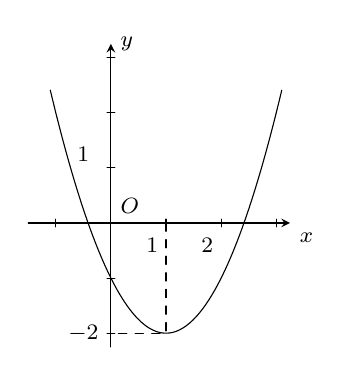
\begin{tikzpicture}[line cap=round,line join=round,font=\footnotesize,>=stealth,scale=0.7]
				 \tikzset{label style/.style={font=\footnotesize}}
				\draw[->] (-1.5,0)--(3.25,0)  node[below right] {$x$};
				\draw[->]  (0,-2.25)--(0,3.25) node[right] {$y$};
				\node (0,0)  [above right]{$ O $};
				\foreach \x in  {-1,1,2,3}
				\draw[shift={(\x,0)},color=black] (0pt,2pt) -- (0pt,-2pt); 
				\node at (.75,-0.4) {$1$}; 
				\node at (1.75,-0.4) {$2$}; 
				\foreach  \y in {-2,-1,1,2,3}
				\draw[shift={(0,\y)},color=black] (2pt,0pt) -- (-2pt,0pt); 
				\node at (-0.5,1.25)  {$1$};
				 \node at (-0.5,-2) {$-2$};
				 \draw[dashed](1,0)--(1,-2)--(0,-2);
				\draw [domain=-1.1:3.1,samples=100]  plot (\x,{(\x)*(\x)-2*(\x) - 1});
			\end{tikzpicture}
		 }
	 \loigiai{
		 Đồ thị cắt trục $Oy$ tại điểm có tung độ bằng $-1\Rightarrow c=-1$. Suy ra $y=ax^2+bx-1$.\\
		Đồ thị nhận $I\left(1;-2\right)$ làm đỉnh nên $\heva{&\dfrac{-b}{2a}=1\\ &-2=a\cdot 1^2+b\cdot 1-1}\Leftrightarrow\heva{&2a+b=0\\  &a+b=-1}\Leftrightarrow\heva{&a=1\\ &b=-2.}$\\
		Vậy $y=x^2-2x-1$. 
	} 
\end{ex}

% nguồn: MaHoaNH_TracNghiem_Lop10
\begin{ex}%[0D3H2-3]%[ma:4d33ccde]
	Cho hàm số  $y=x^2-3x$. Hỏi hình nào sau đây là đồ thị của hàm số đã cho?
	\choice 
		{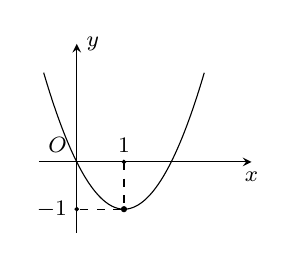
\begin{tikzpicture}[smooth,samples=300,scale=0.6,>=stealth,font=\footnotesize]
		\draw[->] (-0.8,0)--(3.7,0) node[below]{$x$}; 
		\draw[->]  (0,-1.5)--(0,2.5) node[right]{$y$};
		\draw (0,0)  node[above left]{$O$};
		\draw[domain=-0.7:2.7]  plot (\x,{(\x+1)^2-4*(\x+1)+3});
		\draw[fill=black] (1,-1) circle  (1.5pt)
			 (1,0) circle (1pt)
			(0,-1) circle (1pt); 
		\draw[dashed]  (1,0) node[above]{$1$}--(1,-1)--(0,-1) node[left]{$-1$};
	\end{tikzpicture}
		 }
		{\True 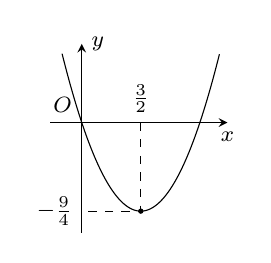
\begin{tikzpicture}[smooth,samples=300,scale=0.5,>=stealth,font=\footnotesize]
		\draw[->] (-0.8,0)--(3.7,0) node[below]{$x$}; 
		\draw[->]  (0,-2.8)--(0,2) node[right]{$y$};
		\draw (0,0)  node[above left]{$O$};
		 \draw[domain=-0.5:3.5] plot (\x,{(\x)^2-3*(\x)});
		\draw[fill=black] (1.5,-2.25) circle (1.5pt); 
		\draw[dashed] (1.5,0) node[above]{$\frac{3}{2}$}--(1.5,-2.25)--(0,-2.25) node[left]{$-\frac{9}{4}$}; 
	\end{tikzpicture}
		} 
		{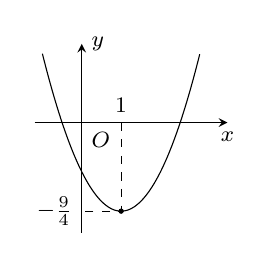
\begin{tikzpicture}[smooth,samples=300,scale=0.5,>=stealth,font=\footnotesize]
		\draw[->]  (-1.2,0)--(3.7,0) node[below]{$x$};
		 \draw[->] (0,-2.8)--(0,2) node[right]{$y$};
		\draw (0,0)  node[below right]{$O$};
		 \draw[domain=-1:3] plot (\x,{(\x+0.5)^2-3*(\x+0.5)});
		\draw[fill=black]  (1,-2.25) circle (1.5pt);
		\draw[dashed]  (1,0) node[above]{$1$}--(1,-2.25)--(0,-2.25) node[left]{$-\frac{9}{4}$};
	\end{tikzpicture}
		 }
		{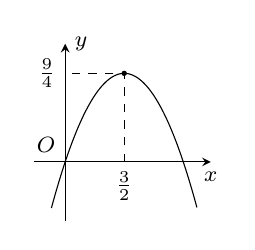
\begin{tikzpicture}[smooth,samples=300,scale=0.5,>=stealth,font=\footnotesize]
		\draw[->] (-0.8,0)--(3.7,0) node[below]{$x$}; 
		\draw[->] (0,-1.5)--(0,3)  node[right]{$y$};
		\draw (0,0) node[above left]{$O$}; 
		\draw[domain=-0.35:3.35]  plot (\x,{-(\x)^2+3*(\x)});
		\draw[fill=black] (1.5,2.25) circle  (1.5pt);
		\draw[dashed] (1.5,0)  node[below]{$\frac{3}{2}$}--(1.5,2.25)--(0,2.25) node[left]{$\frac{9}{4}$};
	\end{tikzpicture}
		} 
	\loigiai{ 
		Tọa độ đỉnh của parabol là $I\left(\dfrac{-b}{2a};\dfrac{-\Delta}{4a}\right)=I\left(\dfrac{3}{2};\dfrac{-9}{4}\right)$. 
	 }
\end{ex}

% nguồn: MaHoaNH_TracNghiem_Lop10
\begin{ex}%[0D3H2-3]%[ma:f70cb732]
	Nếu hàm số $y=ax^2+bx+c$ có $a>0$; $ b>0$ và $c<0$ thì  đồ thị hàm số của nó có dạng
	 \choice
		{\True 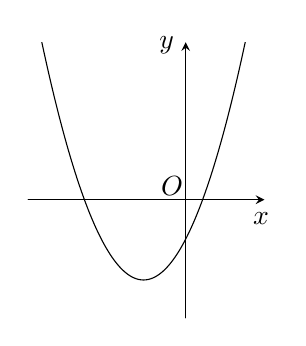
\begin{tikzpicture}[font=\footnotesize,line join=round,line cap=round,>=stealth]
		\tikzset{declare function={xmin=-2;  xmax=1; ymin=-1.5; ymax=2;
			 f (\x)=1.81*(\x)^2+1.94*(\x)-0.5;
			 },
			 smooth,samples=450
		 }
		\draw[->]  (xmin,0)--(xmax,0) node[shift={(-100:7pt)},font=\normalsize]{$ x $};
		\draw[->] (0,ymin)--(0,ymax) node[shift={(190:7pt)},font=\normalsize]{$  y $};
		\fill (0,0) node[shift={(135:7pt)},font=\normalsize]{$ O  $};
		\clip (xmin,ymin) rectangle (xmax,ymax); 
		\draw plot[domain=xmin:xmax] (\x,{f (\x)}); 
	\end{tikzpicture}
		} 
		{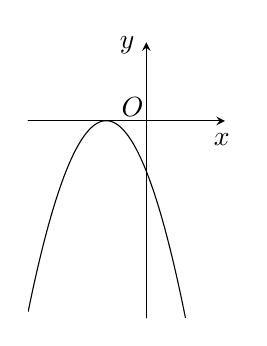
\begin{tikzpicture}[font=\footnotesize,line join=round,line cap=round,>=stealth]
		\tikzset{declare function={xmin=-1.5; xmax=1; ymin=-2.5;  ymax=1;
			f (\x)=-2.47*(\x)^2-2.52*(\x)-0.64; 
			 },
			smooth,samples=450 
		} 
		\draw[->]  (xmin,0)--(xmax,0) node[shift={(-100:7pt)},font=\normalsize]{$ x $};
		\draw[->] (0,ymin)--(0,ymax) node[shift={(190:7pt)},font=\normalsize]{$ y $}; 
		 \fill (0,0) node[shift={(135:7pt)},font=\normalsize]{$ O $};
		\clip  (xmin,ymin) rectangle (xmax,ymax);
		\draw  plot[domain=xmin:xmax] (\x,{f (\x)});
	\end{tikzpicture}
		} 
		{\begin{tikzpicture}[font=\footnotesize,line join=round,line cap=round,>=stealth]
		 \tikzset{declare function={xmin=-1.5; xmax=2.5; ymin=-2; ymax=2.5;
			 f (\x)=-1.3*(\x)^2+1.3*(\x)+1.6;
			 },
			 smooth,samples=450
		} 
		\draw[->] (xmin,0)--(xmax,0)  node[shift={(-100:7pt)},font=\normalsize]{$ x $};
		\draw[->] (0,ymin)--(0,ymax) node[shift={(190:7pt)},font=\normalsize]{$ y  $};
		\fill (0,0) node[shift={(135:7pt)},font=\normalsize]{$  O $};
		 \clip (xmin,ymin) rectangle (xmax,ymax);
		\draw plot[domain=xmin:xmax]  (\x,{f (\x)});
	\end{tikzpicture}
		} 
		{\begin{tikzpicture}[font=\footnotesize,line join=round,line cap=round,>=stealth]
		\tikzset{declare function={xmin=-1; xmax=2;  ymin=-1; ymax=3;
			f  (\x)=1.99*(\x)^2-2.03*(\x)+1.19;
			 },
			smooth,samples=450 
		} 
		\draw[->] (xmin,0)--(xmax,0) node[shift={(-100:7pt)},font=\normalsize]{$ x  $};
		\draw[->]  (0,ymin)--(0,ymax) node[shift={(190:7pt)},font=\normalsize]{$ y $};
		\fill (0,0) node[shift={(135:7pt)},font=\normalsize]{$ O  $};
		 \clip (xmin,ymin) rectangle (xmax,ymax);
		\draw plot[domain=xmin:xmax] (\x,{f  (\x)});
	\end{tikzpicture}
		 }
	\loigiai{ 
		Đồ thị hàm số $a>0$ nên bề lõm đồ thị quay lên và $c<0$ nên đồ thị cắt trục $Oy$ phía dưới $Ox $ nên  ta chọn
		\begin{center}
			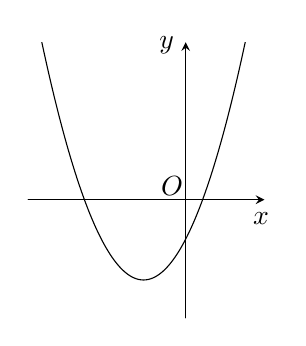
\begin{tikzpicture}[font=\footnotesize,line join=round,line cap=round,>=stealth]
					 \tikzset{declare function={xmin=-2; xmax=1; ymin=-1.5; ymax=2;
						f (\x)=1.81*(\x)^2+1.94*(\x)-0.5; 
						 },
						smooth,samples=450 
					 }
					\draw[->] (xmin,0)--(xmax,0) node[shift={(-100:7pt)},font=\normalsize]{$ x  $};
					\draw[->] (0,ymin)--(0,ymax) node[shift={(190:7pt)},font=\normalsize]{$ y  $};
					\fill  (0,0) node[shift={(135:7pt)},font=\normalsize]{$ O $};
					\clip  (xmin,ymin) rectangle (xmax,ymax);
					\draw  plot[domain=xmin:xmax] (\x,{f (\x)});
				\end{tikzpicture}
		\end{center}
	} 
\end{ex}

% nguồn: MaHoaNH_TracNghiem_Lop10
\begin{ex}%[0D3H2-3]%[ma:06c1e007]
	Hàm số $y=ax^2+bx+c$ với $a>0$; $ b>0$ và $c<0$ có đồ thị là đường  cong nào dưới đây?
	 \choice
		{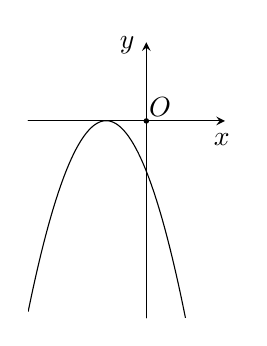
\begin{tikzpicture}[font=\footnotesize,line join=round,line cap=round,>=stealth]
		\tikzset{declare function={xmin=-1.5; xmax=1; ymin=-2.5; ymax=1; 
			f (\x)=-2.47*(\x)^2-2.52*(\x)-0.64; 
			 },
			 smooth,samples=450
		} 
		\draw[->] (xmin,0)--(xmax,0) node[shift={(-100:7pt)},font=\normalsize]{$ x  $};
		 \draw[->] (0,ymin)--(0,ymax) node[shift={(190:7pt)},font=\normalsize]{$ y $};
		\fill  (0,0) node[shift={(45:7pt)},font=\normalsize]{$ O $};
		\fill (0,0) circle  (1pt);
		\clip (xmin,ymin) rectangle (xmax,ymax); 
		\draw plot[domain=xmin:xmax] (\x,{f  (\x)});
	\end{tikzpicture}
		} 
		{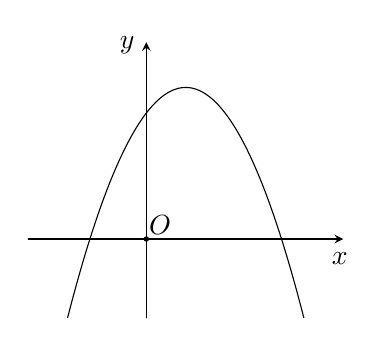
\begin{tikzpicture}[font=\footnotesize,line join=round,line cap=round,>=stealth]
		\tikzset{declare function={xmin=-1.5; xmax=2.5; ymin=-1;  ymax=2.5;
			f (\x)=-1.3*(\x)^2+1.3*(\x)+1.6; 
			 },
			smooth,samples=450 
		 }
		\draw[->] (xmin,0)--(xmax,0) node[shift={(-100:7pt)},font=\normalsize]{$  x $};
		\draw[->] (0,ymin)--(0,ymax) node[shift={(190:7pt)},font=\normalsize]{$ y $}; 
		\fill (0,0) node[shift={(45:7pt)},font=\normalsize]{$ O  $};
		\fill (0,0) circle  (1pt);
		\clip (xmin,ymin) rectangle (xmax,ymax); 
		\draw  plot[domain=xmin:xmax] (\x,{f (\x)});
	\end{tikzpicture}
		 }
		{\True 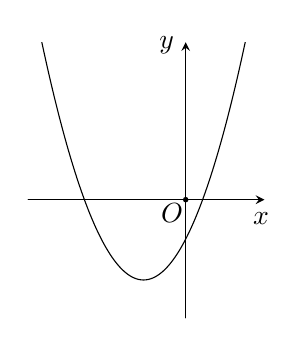
\begin{tikzpicture}[font=\footnotesize,line join=round,line cap=round,>=stealth]
		\tikzset{declare function={xmin=-2; xmax=1; ymin=-1.5;  ymax=2;
			f (\x)=1.81*(\x)^2+1.94*(\x)-0.5; 
			}, 
			smooth,samples=450 
		} 
		\draw[->] (xmin,0)--(xmax,0)  node[shift={(-100:7pt)},font=\normalsize]{$ x $};
		\draw[->] (0,ymin)--(0,ymax) node[shift={(190:7pt)},font=\normalsize]{$ y $}; 
		\fill (0,0)  node[shift={(-135:7pt)},font=\normalsize]{$ O $};
		 \fill (0,0) circle (1pt);
		 \clip (xmin,ymin) rectangle (xmax,ymax);
		\draw plot[domain=xmin:xmax]  (\x,{f (\x)});
	\end{tikzpicture}
		 }
		{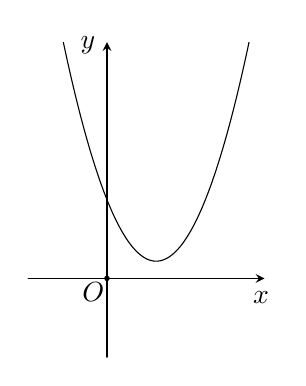
\begin{tikzpicture}[font=\footnotesize,line join=round,line cap=round,>=stealth]
		\tikzset{declare function={xmin=-1; xmax=2; ymin=-1; ymax=3; 
			f (\x)=2*(\x)^2-2.5*(\x)+1; 
			}, 
			smooth,samples=450 
		} 
		\draw[->]  (xmin,0)--(xmax,0) node[shift={(-100:7pt)},font=\normalsize]{$ x $};
		\draw[->] (0,ymin)--(0,ymax) node[shift={(190:7pt)},font=\normalsize]{$  y $};
		 \fill (0,0) node[shift={(-135:7pt)},font=\normalsize]{$ O $};
		\fill (0,0) circle  (1pt);
		\clip (xmin,ymin) rectangle (xmax,ymax); 
		\draw  plot[domain=xmin:xmax] (\x,{f (\x)});
	\end{tikzpicture}
		 }
	 \loigiai{
		Đồ thị hàm số $a>0$ nên bề  lõm đồ thị quay lên và $c<0$ nên đồ thị cắt trục $Oy$ tại điểm có tung độ âm.
		\begin{center}
			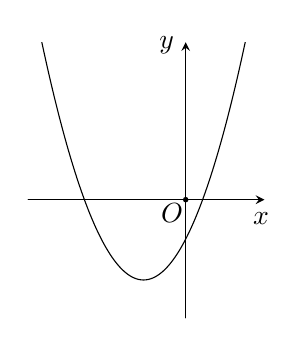
\begin{tikzpicture}[font=\footnotesize,line join=round,line cap=round,>=stealth]
					\tikzset{declare  function={xmin=-2; xmax=1; ymin=-1.5; ymax=2;
						f  (\x)=1.81*(\x)^2+1.94*(\x)-0.5;
						}, 
						smooth,samples=450 
					} 
					 \draw[->] (xmin,0)--(xmax,0) node[shift={(-100:7pt)},font=\normalsize]{$ x $};
					 \draw[->] (0,ymin)--(0,ymax) node[shift={(190:7pt)},font=\normalsize]{$ y $};
					\fill (0,0)  node[shift={(-135:7pt)},font=\normalsize]{$ O $};
					\fill (0,0) circle  (1pt);
					 \clip (xmin,ymin) rectangle (xmax,ymax);
					 \draw plot[domain=xmin:xmax] (\x,{f (\x)});
				\end{tikzpicture}
		\end{center}
	} 
\end{ex}

% nguồn: MaHoaNH_TracNghiem_Lop10
\begin{ex}%[0D3B2-3]%[ma:9ee597ea]
	Cho  hàm số $y=x^2-3 x+2$. Phương trình trục đối xứng của đồ thị hàm số là
	 \choice
		{\True  $x=\dfrac{3}{2}$}
		 {$y=\dfrac{3}{2}$}
		{$y=-\dfrac{3}{2}$} 
		{$x=-\dfrac{3}{2}$} 
	 \loigiai{
		Trục  đối xứng của đồ thị hàm số trên là $x=\dfrac{-b}{2a}=\dfrac{3}{2}$.
	} 
\end{ex}

% nguồn: MaHoaNH_TracNghiem_Lop10
\begin{ex}%[0D3Y2-3]%[ma:b85d720b]
	Trục đối xứng của  đồ thị hàm số $y=x^2+2x-1$ là
	 \choice
		 {\True $x=-1$}
		{$x=1$} 
		{$y=1$} 
		{$y=-1$} 
	 \loigiai{
		Trục đối xứng của đồ thị hàm số là $x=\dfrac{-2}{2 \cdot 1}  \Leftrightarrow x=-1$.
	 }
\end{ex}

% nguồn: MaHoaNH_TracNghiem_Lop10
\begin{ex}%[0D3Y2-3]%[ma:054ab3d7]
	Cho hàm số bậc hai $y=ax^2+bx+c$ $(a \neq 0)$ có đồ thị $(P)$. Đỉnh  của $(P)$ được xác định bởi công thức nào?
	 \choice
		 {$I\left(-\dfrac{b}{a};-\dfrac{\Delta}{4a}\right)$}
		{$I\left(-\dfrac{b}{2a};\dfrac{\Delta}{4a}\right)$} 
		{\True  $I\left(-\dfrac{b}{2a};-\dfrac{\Delta}{4a}\right)$}
		{$I\left(\dfrac{b}{2a};\dfrac{\Delta}{4a}\right)$} 
	\loigiai{ 
		$I\left(-\dfrac{b}{2a};-\dfrac{\Delta}{4a}\right)$ là đỉnh của parabol  $(P) \colon y=ax^2+bx+c$.
	 }
\end{ex}

% nguồn: MaHoaNH_TracNghiem_Lop10
\begin{ex}%[0D3Y2-3]%[ma:afb25811]
	Cho hàm số bậc hai $y=ax^2+bx+c$ $(a \neq 0)$ có đồ thị $(P)$, đỉnh của $(P)$ được xác định bởi công thức nào? 
	\choice 
		 {\True $I\left(-\dfrac{b}{2a};-\dfrac{\Delta}{4a}\right)$}
		 {$I\left(\dfrac{b}{a};\dfrac{\Delta}{4a}\right)$}
		{$I\left(-\dfrac{b}{a};-\dfrac{\Delta}{4a}\right)$} 
		 {$I\left(-\dfrac{b}{2a};-\dfrac{\Delta}{2a}\right)$}
	\loigiai{ 
		Đồ thị hàm số $y=ax^2+bx+c$ $(a \neq 0)$  là parabol có đỉnh $I\left(-\dfrac{b}{2a};-\dfrac{\Delta}{4a}\right)$.
	} 
\end{ex}

% nguồn: MaHoaNH_TracNghiem_Lop10
\begin{ex}%[0D3B2-3]%[ma:73e7f012]
	Cho parabol $(P)\colon y=x^2-2x-3$.  Điểm nào sau đây là đỉnh của $(P)$?
	\choice 
		 {$I(-1; 4)$}
		{\True  $I(1;-4)$}
		 {$I(-1;-4)$}
		{$I(1; 4)$} 
	\loigiai{Hoành độ  đỉnh là $x=-\dfrac{b}{2a}=-\dfrac{-2}{a}=1$.\\
		Với $x=1$, ta  có $y=1-2-3=-4$.\\
		Tọa độ đỉnh  $I(1;-4)$.
	} 
\end{ex}

% nguồn: MaHoaNH_TracNghiem_Lop10
\begin{ex}%[0D3B2-3]%[ma:a06138fc]
	Tìm một đội gồm $ 5 $ nam và $ 8 $ nữ. Lập một nhóm  gồm $ 4 $ người hát tốp ca, tính xác suất để trong $ 4 $ người được chọn có ít nhất $ 3 $ nữ.
	 \choice
		 {$\dfrac{56}{143}$}
		{$\dfrac{87}{143}$} 
		 {\True $\dfrac{70}{143}$}
		{$\dfrac{73}{143}$} 
	\loigiai{ 
		Số phần tử của không gian mẫu  $ \mathrm{C}^4_{13}=715 $.\\
		Số  cách chọn $ 4 $ người có ít nhất $ 3 $ nữ là $ \mathrm{C}^3_8\cdot \mathrm{C}^1_5+\mathrm{C}^4_8=350$.\\
		Vậy xác suất cần tìm là  $ P=\dfrac{70}{143} $.
	} 
\end{ex}

% nguồn: MaHoaNH_TracNghiem_Lop10
\begin{ex}%[0D3B2-3]%[ma:ff4f8bd5]
	Một tổ trong lớp 10A có $4$ bạn nam và $6$ bạn nữ. Giáo viên chọn ngẫu nhiên hai bạn trong tổ để tham gia đội làm báo của  lớp. Xác suất để hai bạn được chọn có một bạn nam và một bạn nữ là?
	\choice 
		 {$\dfrac{2}{15}$}
		{$\dfrac{6}{25}$} 
		{$\dfrac{8}{25}$} 
		 {\True $\dfrac{8}{15}$}
	 \loigiai{
		Ta có $n(\Omega)=\mathrm{C}_{10}^2=45$.\\ 
		Biến cố $A$ \lq\lq Hai  bạn được chọn có một bạn nam và một bạn nữ\rq\rq.\\
		Suy  ra, $n(A)=\mathrm{C}_6^1\cdot\mathrm{C}_4^1=24$.\\
		Vậy xác suất biến cố $A$ là $\mathrm{P}(A)=\dfrac{n(A)}{n(\Omega)}=\dfrac{24}{45}=\dfrac{8}{15}$. 
	} 
\end{ex}

% nguồn: MaHoaNH_TracNghiem_Lop10
\begin{ex}%[0D3B2-3]%[ma:8072c2d8]
	Lớp A có $9$ học sinh xuất sắc, lớp B có $10$ học sinh xuất  sắc. Chọn ngẫu nhiên $2$ trong các học sinh
	đó đi dự lễ tuyên dương học sinh tiêu biểu. Xác suất để $2$ học sinh được chọn từ cùng một  lớp là?
	 \choice
		{$\dfrac{10}{19}$} 
		{\True  $\dfrac{9}{19}$}
		{$\dfrac{13}{18}$} 
		 {$\dfrac{11}{18}$}
	\loigiai{ 
		Ta  có $n(\Omega)=\mathrm{C}_{19}^2=171$.\\
		Biến  cố $A$ \lq\lq$2$ học sinh được chọn từ cùng một lớp\rq\rq.\\
		 Suy ra, $n(A)=\mathrm{C}_{10}^2+\mathrm{C}_9^2=81$.\\
		Vậy xác suất biến cố  $A$ là $\mathrm{P}(A)=\dfrac{n(A)}{n(\Omega)}=\dfrac{81}{171}=\dfrac{9}{19}$.
	 }
\end{ex}

% nguồn: MaHoaNH_TracNghiem_Lop10
\begin{ex}%[0D3B2-3]%[ma:d4413504]
	Một nhóm công nhân gồm $15$ nam và $5$ nữ. Người ta muốn chọn từ nhóm ra  $5$ người để lập thành một tổ công tác gồm một tổ trưởng là nam, một tổ phó là nam và $3$ người còn lại có ít nhất một nữ. Hỏi có bao nhiêu cách lập tổ công tác?
	 \choice
		{\True  $111300$}
		 {$233355$}
		{$109200$} 
		{$112342$} 
	 \loigiai{
		Lấy $2$ nam ra làm tổ trưởng và tổ phó là chỉnh hợp chập $2$ của $15$ phần tử. Lúc này $3$ người còn  lại có ít nhất một nữ sẽ xảy ra các trường hợp sau:
		\begin{itemize}
			\item \textbf{TH1.} $2$ nam và $1$  nữ.
			\item  \textbf{TH2.} $1$ nam và $2$ nữ.
			\item \textbf{TH3.} $3$  nữ.
		\end{itemize}
		Theo đề ta có số cách lập một tổ công tác là $$n(\Omega)=\mathrm{A}_{15}^2 \cdot \mathrm{C}_{13}^2 \cdot  \mathrm{C}_5^1+\mathrm{A}_{15}^2 \cdot \mathrm{C}_{13}^1 \cdot \mathrm{C}_5^2+\mathrm{A}_{15}^2 \cdot \mathrm{C}_5^3=111300.$$
	} 
\end{ex}

% nguồn: MaHoaNH_TracNghiem_Lop10
\begin{ex}%[0D3K2-3]%[ma:45ffd077]
	\immini{ 
	Cho hàm số $y=ax^2+bx+c$ có đồ thị  là parabol trong hình vẽ bên. Khẳng định nào sau đây đúng?
	 \choice
		{\True  $a>0$, $b>0$, $c<0$}
		{$a>0$,  $b>0$, $c>0$}
		 {$a>0$, $b<0$, $c>0$}
		{$a>0$, $b<0$, $c<0$}} 
		{\vspace{-0.5cm} 
		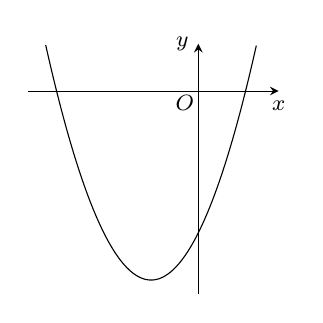
\begin{tikzpicture}[scale=0.6,font=\footnotesize,samples=200,>=stealth]
				\draw[->] (-3.6,0)--(1.7,0) node[below]{$x$}; 
				 \draw[->] (0,-4.3)--(0,1) node[left]{$y$};
				 \node at (0,0) [below left=-2pt]{$O$};
				 \draw plot[domain=-3.23:1.23](\x,{(\x)^2+2*\x-3});
			\end{tikzpicture}
		 }
	 \loigiai{
		Pababol trong hình vẽ có bề lõm  quay lên nên $a>0$, cắt trục hoành tại điểm $A(0;c)$ phía dưới $O$ nên $c<0$.\\
		Ngoài ra trục đối xứng của parabol $x=-\dfrac{b}{2a}$ nằm bên trái trục tung nên $b$ và $a$ cùng dấu nhau, do  đó $b>0$.\\
		 Vậy $a>0$, $b>0$, $c<0$.
	} 
\end{ex}

% nguồn: MaHoaNH_TracNghiem_Lop10
\begin{ex}%[0D3K2-3]%[ma:6c57620d]
	 Đồ thị dưới đây là của hàm số nào?
	\begin{center}
		\begin{tikzpicture}[scale=0.85,>=stealth,font=\footnotesize,line join=round,line cap=round]
				\def\xmin{-2}  \def\xmax{5}
				 \def\ymin{-2} \def\ymax{6}
				\draw[->] (\xmin,0)--(\xmax,0)  node [below]{$x$};
				\draw[->] (0,\ymin)--(0,\ymax) node [left]{$y$}; 
				\node at (0,0) [below left]{$O$}; 
				\clip (\xmin+0.1,\ymin+0.1)  rectangle (\xmax-0.5,\ymax-0.1);
				\draw[smooth,samples=300,domain=-1.5:4.5] plot  (\x,{(\x)^2-4*(\x)+3});
				\draw[dashed] (2,-2)--(2,5) 
					 (0,-1)--(2,-1);
				\draw (-1,0) node[below]  {$-1$}
					 (1,0) node[below left] {$1$}
					(2,0) node  [below right] {$2$}
					(3,0) node[below  right] {$3$}
					(4,0) node[below]  {$4$};
				 \draw (0,-1) node[left] {$-1$}
					(0,1) node[left]  {$1$}
					(0,2) node  [left] {$2$}
					(0,3) node[left] {$3$} 
					 (0,4) node[right] {$4$};
			\end{tikzpicture}
	\end{center}
	\choice 
		{$y=x^2-4x-1$} 
		 {\True $y=x^2-4x+3$}
		 {$y=-x^2+4x-1$}
		 {$y=-x^2+4x+3$}
	 \loigiai{
		Parabol  có bề lõm hướng lên trên nên $a>0$, hơn nữa parabol cắt $Oy$ tại điểm $(0;3)$ nên $c=3$. Do đó đồ thị trong hình vẽ là đồ thị của hàm số $y=x^2-4x+3$.
	} 
\end{ex}

% nguồn: MaHoaNH_TracNghiem_Lop10
\begin{ex}%[0D3B2-3]%[ma:2e05139d]
	Sắp xếp $ 12 $ học sinh lớp $ 10 $ gồm có $ 6 $ học sinh nam, $ 6 $ học sinh nữ vào một bàn dài gồm có hai dãy ghế đối diện nhau (mỗi dãy có $ 6 $ ghế) để thảo luận. Tính xác suất để hai học sinh ngồi đối diện và cạnh  nhau luôn khác giới?
	\choice 
		 {$\dfrac{1}{924}$}
		{\True $\dfrac{1}{462}$} 
		 {$\dfrac{3}{9920}$}
		{$\dfrac{1}{665280}$} 
	\loigiai{ 
		Đánh số vị trí ngồi của hai dãy ghế  đối diện nhau như hình vẽ.
		\begin{center}
			\begin{tabular}{|c|c|c|c|c|c|}
				 \hline
				1 & 2 & 3  & 4 & 5 & 6 \\
				\hline 
				7 & 8 & 9 & 10  & 11 & 12 \\
				 \hline
			\end{tabular}
		\end{center}
		Số phần tử  không gian mẫu bằng số cách xếp $ 12 $ học sinh nên ta có $ 12! $ cách.\\
		Để xếp hai học sinh ngồi đối diện và cạnh nhau luôn khác giới ta làm như sau:\begin{itemize}
		\item Xếp học sinh ở vị trí $ 1 $ có $ 12  $ cách.
		\item Xếp ở vị trí $ 7 $  có $ 6 $ cách.
		\item Xếp ở  vị trí $ 2 $ có $ 5 $ cách.
		\item Xếp ở vị trí $ 8  $ có $ 5 $ cách.
		\item Xếp ở vị trí $ 3  $ có $ 4 $ cách.
		 \item Xếp ở vị trí $ 9 $ có $ 4 $ cách.
		\item Xếp ở vị  trí $ 4 $ có $ 3 $ cách.
		\item Xếp ở vị trí $  10 $ có $ 3 $ cách.
		 \item Xếp ở vị trí $ 5 $ có $ 2 $ cách.
		\item  Xếp ở vị trí $ 11 $ có $ 2 $ cách.
		\item Xếp ở vị trí $ 6 $ có $ 1  $ cách.
		\item Xếp ở  vị trí $ 12 $ có $ 1 $ cách.
	\end{itemize}
	Vậy xác suất cần tìm là $ P=\dfrac{1^2\cdot2^2\cdot3^2\cdot4^2\cdot5^2\cdot6\cdot 12}{12!}=  \dfrac{1}{462}$.
 }
\end{ex}

% nguồn: MaHoaNH_TracNghiem_Lop10
\begin{ex}%[0D3Y2-3]%[ma:46c0a228]
	Cho hàm số $y=x^2-3x$. Hỏi hình nào sau  đây là đồ thị của hàm số đã cho?
	\choice 
		{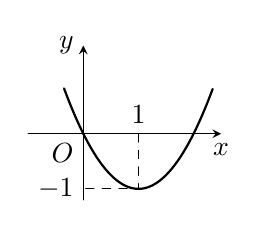
\begin{tikzpicture}[>=stealth,scale=0.7,line join=round,line cap=round]
		\draw[->]  (-1,0)--(2.5,0) node [below]{$x$};
		\draw[->]  (0,-1.2)--(0,1.6) node [left]{$y$};
		\node at  (0,0) [below left]{$O$};
		\clip; 
		\draw[smooth,samples=300,domain=-0.35:2.35,thick]  plot (\x,{(\x)^2-2*(\x)});
		\draw[dashed](1,0) node[above]{$1$}--(1,-1)--(0,-1) node[left]{$-1$}; 
	\end{tikzpicture}
		} 
		{\True 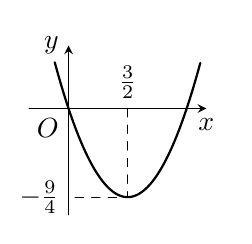
\begin{tikzpicture}[>=stealth,scale=0.5,line join=round,line cap=round]
		\draw[->] (-1,0)--(3.5,0) node [below]{$x$}; 
		 \draw[->] (0,-2.7)--(0,1.6) node [left]{$y$};
		\node at (0,0) [below left]{$O$}; 
		\clip; 
		 \draw[smooth,samples=300,domain=-0.35:3.35,thick] plot (\x,{(\x)^2-3*(\x)});
		\draw[dashed](3/2,0)  node[above]{$\frac{3}{2}$}--(3/2,-9/4)--(0,-9/4) node[left]{$-\frac{9}{4}$};
	\end{tikzpicture}
		 }
		{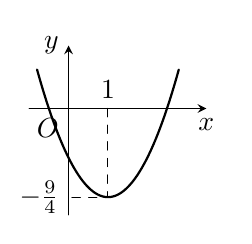
\begin{tikzpicture}[>=stealth,scale=0.5,line join=round,line cap=round]
		 \draw[->] (-1,0)--(3.5,0) node [below]{$x$};
		\draw[->] (0,-2.7)--(0,1.6) node [left]{$y$}; 
		\node at (0,0)  [below left]{$O$};
		\clip; 
		\draw[smooth,samples=300,domain=-0.8:2.8,thick] plot (\x,{(\x)^2-2*(\x)-5/4}); 
		\draw[dashed](1,0)  node[above]{$1$}--(1,-9/4)--(0,-9/4) node[left]{$-\frac{9}{4}$};
	\end{tikzpicture}
		} 
		{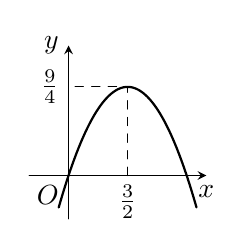
\begin{tikzpicture}[>=stealth,scale=0.5,line join=round,line cap=round]
		 \draw[->] (-1,0)--(3.5,0) node [below]{$x$};
		\draw[->] (0,-1.1)--(0,3.3) node [left]{$y$}; 
		\node at (0,0) [below  left]{$O$};
		\clip; 
		\draw[smooth,samples=300,domain=-0.25:3.25,thick]  plot (\x,{-(\x)^2+3*(\x)});
		\draw[dashed](3/2,0) node[below]{$\frac{3}{2}$}--(3/2,9/4)--(0,9/4)  node[left]{$\frac{9}{4}$};
	\end{tikzpicture}
		 }
	 \loigiai{
		Đồ thị hàm số $y=x^2-3x$ có $a=1>0$ và đỉnh  có tọa độ là $\left(\dfrac{3}{2}; -\dfrac{9}{4}\right)$ nên ta chọn phương án parabol có bề lõm hướng lên và đỉnh có tọa độ là $\left(\dfrac{3}{2}; -\dfrac{9}{4}\right)$.
	} 
\end{ex}


%%%%%%%%%%%%%%%% ĐÚNG/SAI %%%%%%%%%%%%%%%%

% nguồn: MaHoaNH_DungSai_Lop10
\begin{ex}%[0D3N2-3]%[ma:0688d302]
	Cho hàm số $y=-x^2+2x+3$. Các mệnh đề sau đúng hay  sai?
	\choiceTF 
		{\True Tập xác định của hàm số là $\mathscr{D}=\mathbb{R}$} 
		{Tọa độ đỉnh  $I(1;2)$}
		 {Đồ thị hàm số có trục đối xứng là đường thẳng $x=2$}
		 {\True Đồ thị hàm số là Parabol có bề lõm hướng xuống dưới}
	 \loigiai{
		Hàm số $y=-x^2+2x+3$ có $a=-1$, $b=2$, $c=3$. 
		\begin{itemchoice}
			\itemch Tập xác định của hàm số là $\mathscr{D}=\mathbb{R}$  đúng.
			\itemch Tọa độ đỉnh $x_I=-\dfrac{b}{2a}=1$; $y_I=-1^2+2\cdot 1+3=4\Rightarrow  I(1;4)$ sai.
			\itemch Đồ  thị hàm số có trục đối xứng là đường thẳng $x=1$ sai.
			\itemch Vì $a=-1<0$ nên đồ thị hàm số là Parabol có  bề lõm hướng xuống dưới đúng.
		\end{itemchoice}
	 }
\end{ex}

% nguồn: MaHoaNH_DungSai_Lop10
\begin{ex}%[0D3N2-3]%[ma:eff68995]
	Cho hàm số  bậc hai $y=f(x)$ có đồ thị như hình vẽ
	\begin{center}
		\begin{tikzpicture}[>=stealth,x=1.0cm,y=1.0cm,scale=0.8]
				 \draw[->] (-3,0) -- (1,0) node[right] {\footnotesize $x$};
				\draw[->] (0,-2) --  (0,4) node[left] {\footnotesize $y$};
				 \draw (0,0) node[below right] {\footnotesize $O$};
				\draw[line width=1pt,smooth,domain=-3.13:0.13] plot (\x,{2*(\x)^2+6*\x+3}); 
				\draw[dashed] (-1.5,0) node[above]{\footnotesize $-\dfrac{3}{2}$}--(-1.5,-1.5)  node[below]{\footnotesize $I$}--(0,-1.5) node[right]{\footnotesize $-\dfrac{3}{2}$};
				\fill[black] (-1.5,-1.5) circle (2pt); \draw  (0,3) node[right]{\footnotesize $3$};
			\end{tikzpicture}
	\end{center}
	Các khẳng định  sau đây đúng hay sai?
	\choiceTF 
		{\True Đồ thị hàm số có  trục đối xứng $x= -\dfrac{3}{2}$}
		 {Đồ thị hàm số cắt trục tung tại điểm $(3;0)$}
		{\True Đồ thị hàm số có  đỉnh $I\left(-\dfrac{3}{2}; -\dfrac{3}{2}\right)$}
		{\True Hàm số đồng  biến trên $(0;+\infty)$}
	\loigiai{ 
		\begin{itemchoice}
			\itemch Đồ thị hàm số có trục đối xứng $x= -\dfrac{3}{2}$. 
			\itemch Đồ thị hàm số  cắt trục tung tại điểm $(0;3)$.
			\itemch Đồ thị hàm  số có đỉnh $I\left(-\dfrac{3}{2}; -\dfrac{3}{2}\right)$
			\itemch Hàm số đồng biến trên  $(0;+\infty)$.
		\end{itemchoice}
	} 
\end{ex}

% nguồn: MaHoaNH_DungSai_Lop10
\begin{ex}%[0D3H2-3]%[ma:2ef58404]
	\immini{Cho hàm số $y=ax^2+bx+c$ có đồ  thị như hình bên. Xét tính đúng - sai của các khẳng định bên dưới.
	\choiceTF 
		{\True Hàm số nghịch  biến trên $(-\infty;0)$}
		{\True Đồ thị  hàm số cắt trục tung tại đúng một điểm}
		{Phương trình $ax^2+bx+c=0$ có hai nghiệm phân biệt} 
		{\True $ y>0,\forall  x\in\mathbb{R}$}}{
		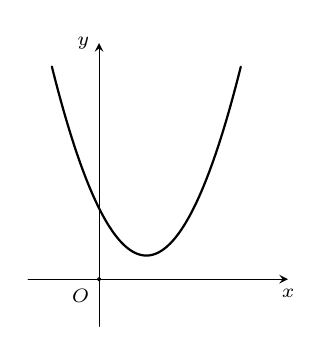
\begin{tikzpicture}[scale=0.6,font=\footnotesize,line join=round,line cap=round,>=stealth]
				\draw[->]  (-1.5,0) -- (4,0) node[below] {\scriptsize $x$};
				\draw[->] (0,-1) -- (0,5) node[left] {\scriptsize  $y$};
				\draw (0,0) circle (1pt)  node[below left]{\scriptsize $O$};
				\draw[thick,samples=150,smooth,domain=-1:3] plot  (\x,{(\x)^2-2*\x+1.5});
			\end{tikzpicture}
		} 
	\loigiai{\begin{itemchoice}
		\itemch Đúng vì đồ thị đi xuống theo chiều từ  trái sang phải trên khoảng $(-\infty;0)$.
		\itemch Đúng vì  đồ thị hàm số cắt trục $Oy$ tại đúng một điểm.
		\itemch Sai vì đồ thị hàm số không cắt trục  $Ox$.
		\itemch Đúng vì đồ thị hàm số nằm phía trên trục $Ox$ và không có  điểm chung với $Ox$ nên $ y>0,\forall x\in\mathbb{R}$.
\end{itemchoice}}
\end{ex}

% nguồn: MaHoaNH_DungSai_Lop10
\begin{ex}%[0D3H2-3]%[ma:41453174]
	Cho tam thức bậc hai $f(x)=x^2-2(m-1)x+m+5$,  với $m$ là tham số. Khi đó
	\choiceTF 
		{\True Khi $m=4$, $f(x)$  có một nghiệm là $x=3$}
		 {\True Điều kiện để $f(x)$ luôn có hai nghiệm phân biệt là $m<-1$ hoặc $m>4$}
		{ Khi  $m=-1$ thì $f(x)>0,\forall x\in \mathbb{R}$}
		{Có $4$ giá trị nguyên của tham số $m$ để bất phương trình $\dfrac{f(x)}{x^2+x+3}\geq 0$ nghiệm đúng với mọi $x\in  \mathbb{R}$}
	 \loigiai{
		\begin{itemchoice}
			 \itemch
			Khi $m=4\Rightarrow f(x)=x^2-6x+9$.  Thay $x=3$ ta được $f(x)=3^2-6\cdot3+9=0$.\\
			Vậy $f(x)$ có một nghiệm  là $x=3$.
			 \itemch
			Để $f(x)$ luôn có hai nghiệm phân  biệt thì
			\[\Delta '=(m-1)^2-m-5>0 \Leftrightarrow m^2-3m-4>0\Leftrightarrow \hoac{&m<-1\\&m>4.}\] 
			Vậy điều kiện để $f(x)$ luôn có hai nghiệm phân biệt  là $m<-1$ hoặc $m>4$.
			\itemch 
			Khi $m=-1\Rightarrow f(x)=x^2+4x+4=(x+2)^2>0,\ \forall  x \neq -2$.
			\itemch 
			Ta có $x^2+x+3>0,\, \forall  x \in \mathbb{R}$.\\
			Từ 
			$\dfrac{f(x)}{x^2+x+3}\geq 0\Leftrightarrow f(x)\geq 0,\, \forall  x\in \mathbb{R} \Leftrightarrow m^2-3m-4\leq 0\Leftrightarrow -1\leq m\leq 4$.\\
			Các giá  trị nguyên của $m$ là $m\in \{-1;0;1;2;3;4\}$.
		\end{itemchoice}
	} 
\end{ex}

% nguồn: MaHoaNH_DungSai_Lop10
\begin{ex}%[0D3H2-3]%[ma:1b76dda1]
	Cho hàm số bậc hai $y=ax^2+bx+c$ có đồ thị như  hình vẽ
	\begin{center}
		\begin{tikzpicture}[>=stealth,x=1cm,y=1cm,scale=0.6]
				\begin{scriptsize}
					\def\xmin{-4} \def\xmax{2}  \def\ymin{-3.5} \def\ymax{2};
					 \draw [->] (\xmin-.2,0)--(\xmax+.2,0) node[below]{$x$};
					\draw [->] (0,\ymin-.2)--(0,\ymax+.2)  node[right]{$y$};
					\draw  node [below left]{$O$};
					\draw[smooth,domain=-3.25:1.25] plot (\x,{(\x)^(2)+2*(\x)-2}); 
				\end{scriptsize}
			\end{tikzpicture}
	\end{center}
	 Các khẳng định sau đây đúng hay sai?
	\choiceTF 
		{\True  $a>0$}
		{$b<0$} 
		{$c>0$} 
		 {\True $4ac-b^2 <0$}
	\loigiai{ 
		\begin{itemchoice}
			 \itemch Từ đồ thị hàm số ta thấy $a>0$.
			\itemch Trục đối xứng nằm bên trái  nên $-\dfrac{b}{2a} <0 \Rightarrow b>0$.
			\itemch Đồ thị cắt trục tung tại điểm  nằm dưới trục hoành nên $c<0$.
			\itemch Đồ thị cắt trục hoành tại hai điểm phân biệt nên $\Delta >0 \Leftrightarrow b^2-4ac >0$. 
		\end{itemchoice}
	 }
\end{ex}

% nguồn: MaHoaNH_DungSai_Lop10
\begin{ex}%[0D3H2-3]%[ma:c8fc4d37]
	Cho hàm số bậc  hai $y=f(x)=ax^2+bx+c$ có đồ thị như hình dưới
	\begin{center}
		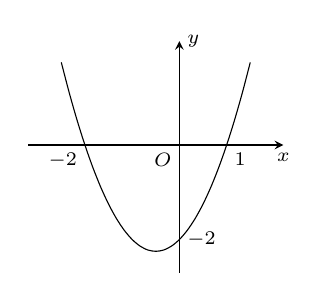
\begin{tikzpicture}[>=stealth,x=1cm,y=1cm,scale=0.6]
				\begin{scriptsize}
					 \def\xmin{-3} \def\xmax{2} \def\ymin{-2.5} \def\ymax{2};
					\draw [->]  (\xmin-.2,0)--(\xmax+.2,0) node[below]{$x$};
					\draw [->] (0,\ymin-.2)--(0,\ymax+.2)  node[right]{$y$};
					\draw  node [below left]{$O$};
					\draw (-2,0) node  [below left]{$-2$}
						(1,0)  node [below right]{$1$}
						(0,-2)  node [right]{$-2$};
					\draw[smooth,domain=-2.5:1.5] plot (\x,{(\x)^(2)+(\x)-2}); 
				\end{scriptsize}
			\end{tikzpicture}
	\end{center}
	Các khẳng định  sau đây đúng hay sai?
	\choiceTF 
		{\True  $c=-2$}
		{Hàm số nghịch biến trên $(-\infty;  0)$}
		{$b<0$} 
		{\True Hàm số đạt giá trị nhỏ nhất bằng $-\dfrac{9}{4}$} 
	\loigiai{ 
		\begin{itemchoice}
			\itemch Đồ thị hàm số cắt trục tung tại  $-2$ nên $c=-2$.
			\itemch Hàm  số không nghịch biến trên $(-\infty;0)$.
			\itemch Đồ thị hàm  số cắt trục hoành tại $x=-2$; $x=1$ nên $f(x)= a(x+2)(x-1) = ax^2+ax -2a$. \\
			$c=-2 \Leftrightarrow -2a =  -2 \Leftrightarrow a=1$. Suy ra $f(x) = x^2+x-2$. \\
			Hàm số  $f(x)$ tại giá trị nhỏ nhất bằng $-\dfrac{9}{4}$ tại $x=-\dfrac{1}{2}$.
		\end{itemchoice}
	 }
\end{ex}

% nguồn: MaHoaNH_DungSai_Lop10
\begin{ex}%[0D3H2-3]%[ma:379273a5]
	 \immini[thm]{
	Cho đồ thị hàm số bậc hai $y=f(x)$ có dạng  như hình sau
	 \choiceTF
		{Trục đối xứng của đồ thị là  đường thẳng $x=-2$}
		{\True Đỉnh  $I$ của đồ thị hàm số có tọa độ là $(2;-2)$}
		{\True Đồ thị hàm  số đi qua điểm $A(0; 6)$}
		{Hàm số đã cho là $y=2  x^2-2 x+6$}
		 }{
		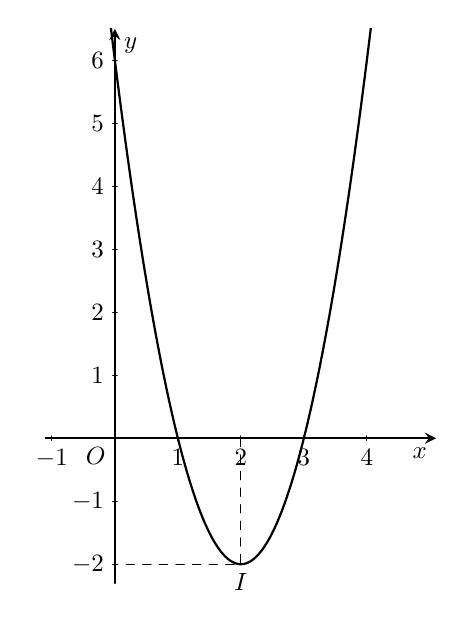
\begin{tikzpicture}[line join=round,line cap=round,>=stealth,thick,scale=0.8]
				 \tikzset{every node/.style={scale=0.9}}
				\draw[->] (-1.1,0)--(5.1,0) node[below  left] {$x$};
				\draw[->] (0,-2.3)--(0,6.5) node[below right] {$y$}; 
				\draw  (0,0) node [below left] {$O$};
				\foreach  \x/\nx in {-1/-1,1/1,2/2,3/3,4/4}
				\draw[thin] (\x,1pt)--(\x,-1pt)  node [below] {$\nx$};
				 \foreach \y/\ny in {-2/-2,-1/-1,1/1,2/2,3/3,4/4,5/5,6/6}
				\draw[thin] (1pt,\y)--(-1pt,\y) node [left] {$\ny$}; 
				 \draw[dashed,thin](2,0)--(2,-2)--(0,-2);
				\draw (2,-2)  node [below] {$I$};
				\begin{scope}
					 \clip (-1,-2.5) rectangle (5,6.5);
					\draw[samples=200,domain=-1:5,smooth,variable=\x] plot (\x,{2*(\x)^2+-8*(\x)+6}); 
				\end{scope}
			\end{tikzpicture}
		 }
	 \loigiai{
		\begin{itemchoice}
			\itemch Sai. Trục đối xứng của đồ thị là đường thẳng  $x=2$.
			\itemch Đúng. Đỉnh $I$ của đồ thị hàm số  có tọa độ là $(2;-2)$.
			\itemch Đúng. Đồ thị hàm số đi qua  điểm $A(0; 6)$.
			\itemch  Sai. Do đồ thị hàm số đi qua điểm $A(0; 6)$ nên $a \cdot 0^2+b \cdot 0+c=6 \Rightarrow c=6$.\\
			 Mặt khác, đồ thị có tọa độ đỉnh là $I(2;-2)$ nên ta có
			$$\heva{&-\dfrac { b }{ 2 a } = 2\\&a \cdot 2 ^ { 2 } + b \cdot  2 + 6 = - 2}\Leftrightarrow \heva{&4 a + b = 0\\&4 a + 2 b = - 8}\Leftrightarrow \heva{&a=2\\&b=-8.}$$
			Vậy hàm số đã cho là  $y=2 x^2-8 x+6$.
		\end{itemchoice}
	 }
\end{ex}

% nguồn: MaHoaNH_DungSai_Lop10
\begin{ex}%[0D3V2-3]%[ma:4745372d]
	\immini[thm]{ 
	 Quan sát đồ thị hàm số bậc hai $y=f(x)$ ở hình bên. Khi đó
	\choiceTF 
		{\True  $a>0$}
		{\True Toạ độ đỉnh $I(2;-1)$, trục đối  xứng $x=2$}
		 {Đồng biến trên khoảng $(-\infty; 2)$; Nghịch biến trên khoảng $(2;+\infty)$}
		{\True $x$ thuộc các khoảng $(-\infty;  1)$ và $(3;+\infty)$ thì $f(x)>0$}
		 }{
		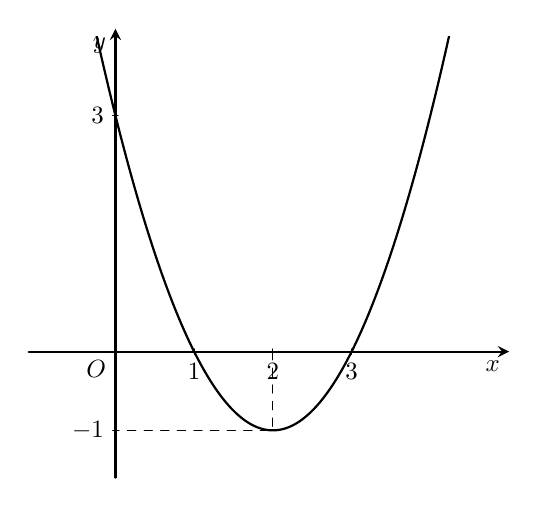
\begin{tikzpicture}[line join=round,line cap=round,>=stealth,thick]
				\tikzset{every node/.style={scale=0.9}} 
				\draw[->] (-1.1,0)--(5,0) node[below  left] {$x$};
				\draw[->]  (0,-1.6)--(0,4.1) node[below left] {$y$};
				\draw (0,0) node [below left]  {$O$};
				\foreach \x/\nx  in {1/1,2/2,3/3}
				\draw[thin]  (\x,1pt)--(\x,-1pt) node [below] {$\nx$};
				\foreach \y/\ny in {-1/-1,3/3} 
				\draw[thin] (1pt,\y)--(-1pt,\y) node [left] {$\ny$}; 
				 \draw[dashed,thin](2,0)--(2,-1)--(0,-1);
				\begin{scope}
					\clip  (-1,-1.5) rectangle (5,4);
					 \draw[samples=200,domain=-1:5,smooth,variable=\x] plot (\x,{1*(\x)^2+-4*(\x)+3});
				\end{scope}
			\end{tikzpicture}
		 }
	 \loigiai{
		\begin{itemchoice}
			\itemch Đúng.  Bề lõm quay lên nên $a>0$.
			\itemch Đúng. Toạ  độ đỉnh $I(2;-1)$, trục đối xứng $x=2$.
			 \itemch Sai. Đồng biến trên khoảng $(2;+\infty)$; nghịch biến trên khoảng $(-\infty; 2)$.
			\itemch Đúng. Vì $x$ thuộc các  khoảng $(-\infty; 1)$ và $(3;+\infty)$ thì $f(x)>0$.
		\end{itemchoice}
	} 
\end{ex}


%%%%%%%%%%%%%%%% TRẢ LỜI NGẮN %%%%%%%%%%%%%%%%

% nguồn: MaHoaNH_TraLoiNgan_Lop10
\begin{bt}%[0D3H2-3]%[ma:073cc5cc]
	Biết đồ thị hàm số $y=ax^2+bx+c$, ($a, b,c \in\mathbb{R}; a\neq  0$) đi qua điểm $A(2;1)$ và có đỉnh $I(1;-1)$. Tính giá trị biểu thức $\mathrm{T}=a^3+b^2-2c$.
	 \shortans{22}
	\loigiai{ 
		$(P)\colon y=ax^2+bx+c$.\\ 
		$(P)$ qua  $A(2;1)\Leftrightarrow 4a+2b+c=1$. \qquad (1)\\
		$(P)$ có đỉnh $I(1;-1)\Rightarrow  \heva{&a+b+c=-1\\&-\dfrac{b}{2a}=1}\Leftrightarrow\heva{&a+b+c=-1&\qquad(2)\\&2a+b=0.&\qquad(3)}$\\
		Từ $(1)$, $(2)$, $(3)$ suy ra  $\heva{&a=2\\&b=-4\\&c=1.}$\\
		 Vậy $T=a^3+b^2-2c=2^3+(-4)^2-2\cdot 1=22$.
	 }
\end{bt}

% nguồn: MaHoaNH_TraLoiNgan_Lop10
\begin{bt}%[0D3V2-3]%[ma:4ab0ed62]
	Biết parabol $(P)\colon y = ax^2 + bx + c$ đi qua hai điểm $A(2;1)$ và $B(-3;5)$. Tính giá trị  của biểu thức $S=44a-8b+6c+3$.
	\shortans{25} 
	\loigiai{ 
		Vì $(P)$ đi qua  hai điểm $A, B$ nên ta có $\heva{&4a+2b+c=1\\&9a-3b+c=5}\Leftrightarrow \heva{&8a+4b+2c=2\\&36a-12b+4c=20.}$\\
		Cộng vế  theo vế ta được $44a-8b+6c=22$ suy ra $S=25$.
	} 
\end{bt}


%%%%%%%%%%%%%%%% TỰ LUẬN %%%%%%%%%%%%%%%%

% nguồn: MaHoaNH_TuLuan_Lop10
\begin{bt}%[0D3H2-3]%[ma:512b7d98]
	 \immini[thm]{
	Cho hàm số bậc  hai $y=ax^2+bx+c$ có đồ thị như hình vẽ sau. Tính giá trị của $a-b^2+c^3$
	 }{
	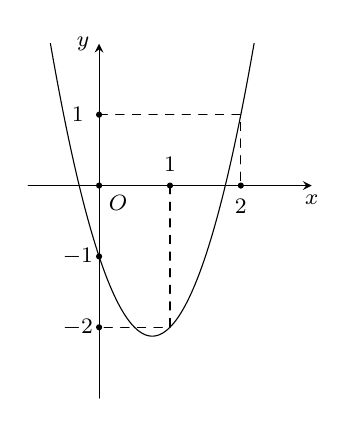
\begin{tikzpicture}[scale=0.9,font=\footnotesize,line join=round,line cap=round,>=stealth]
			 \def\a{2}
			 \def\b{-3}
			\def\c{-1} 
			\draw[->] (-1,0) --  (3,0) node[below] {$x$};
			 \draw[->] (0,-3) -- (0,2) node[left] {$y$};
			\draw[fill=black] (0,0) circle  (1pt) node[below right]{$O$};
			\clip (-1,-3)  rectangle (3,2);
			\draw[samples=150,smooth,domain=-1:2.2] plot  (\x,{\a*(\x)^2+(\b)*(\x)+(\c)});
			 \draw[dashed] (0,1)-|(2,0)
				 (1,0)|-(0,-2);
			\foreach \i/\g  in {1/90,2/-90} \draw[fill=black] (\i,0) circle (1pt) ++(\g:0.3) node{$\i$};
			\foreach \j/\g in  {-1/180,-2/180,1/180} \draw[fill] (0,\j) circle (1pt) ++(\g:0.3) node{$\j$};
		\end{tikzpicture}
	 }
	 \loigiai{
		Khi $x=1$ thì  $y=-2\Rightarrow a+b+c=-2$.\\
		Khi $x=2$  thì $y=1\Rightarrow 4a+2b+c=1$.\\
		Đồ thị cắt trục tung tại điểm có tung độ bằng  $-1$ nên $c=-1$.\\
		Ta có hệ phương  trình $\heva{&c=-1\\&a+b+c=-2\\&4a+2b+c=1} \Leftrightarrow\heva{&a=2\\&b=-3\\&c=-1.} \Rightarrow a-b^2+c^3=-8$
	} 
\end{bt}

% nguồn: MaHoaNH_TuLuan_Lop10
\begin{bt}%[0D3B2-3]%[ma:715d78e0]
	Lớp 10A8 có $10$ bạn nữ và $20$ bạn nam. Thầy giáo chủ nhiệm cần chọn ra $5$ bạn để biên tập Video giới thiệu về lớp mình. Tính xác  suất để thầy có thể chọn được
	\begin{enumerate}
		\item $2$ bạn nam và $3$  bạn nữ.
		\item Có nhiều nhất $1$  bạn nam.
	\end{enumerate}
	\loigiai{ 
		Ta có $n(\Omega)=\mathrm{C}_{30}^5$. 
		\begin{enumerate}
			\item Gọi $A$ là biến cố  \lq\lq Chọn được $2$ bạn nam và $3$ bạn nữ\rq\rq.
			Ta  có $n(A)=\mathrm{C}_{20}^2\cdot\mathrm{C}_{10}^3$.\\
			Khi đó, xác suất của  biến cố $A$ là $\mathrm{P}(A)=\dfrac{n(A)}{n(\Omega)}=\dfrac{\mathrm{C}_{20}^2\cdot\mathrm{C}_{10}^3}{\mathrm{C}_{30}^5}=\dfrac{3800}{23751}$.
			\item Gọi $B$  là biến cố \lq\lq Có nhiều nhất $1$ bạn nam\rq\rq.
			\begin{itemize}
				\item Chọn  $5$ bạn nữ có $\mathrm{C}_{10}^5$ cách.
				\item Chọn  $1$ bạn nam và $4$ bạn nữ có $\mathrm{C}_{20}^1\cdot\mathrm{C}_{10}^4$ cách.
			\end{itemize}
			Ta có  $n(B)=\mathrm{C}_{10}^5+\mathrm{C}_{20}^1\cdot\mathrm{C}_{10}^4=4452$.\\
			Khi  đó, xác suất của biến cố $B$ là $\mathrm{P}(B)=\dfrac{n(B)}{n(\Omega)}=\dfrac{4452}{\mathrm{C}_{30}^5}=\dfrac{106}{3393}$.
		\end{enumerate}
	} 
\end{bt}

% nguồn: MaHoaNH_TuLuan_Lop10
\begin{bt}%[0D3B2-3]%[ma:f69855d3]
	Cho hàm số $y=-2x^2+6x$  có đồ thị $(P)$.
	\begin{listEX}[1]
		\item Vẽ  đồ thị $(P)$.
		\item Tìm toạ độ giao  điểm của $(P)$ với trục hoành.
	\end{listEX}
	\loigiai{ 
		\begin{listEX}
			\item Vẽ đồ thị  $(P)$
			\begin{itemize}
				 \item Tọa độ đỉnh $S\left(\dfrac{3}{2};\dfrac{9}{2}\right)$.
				\item Trục  đối xứng $x=\dfrac{3}{2}$.
				 \item Bảng giá trị
				\begin{center}
					\begin{tabular}{|c|c|c|c|c|c|c|}
						 \hline
						$x$ &  $0$ &$1$ & $\tfrac{3}{2}$&$2$ &$3$\\
						 \hline
						$y=-2x^2+6x$ & $0$ & $4$ &$\tfrac{9}{2}$  & $2$ & $0$\\
						 \hline
					\end{tabular}
				\end{center}
				\item Đồ thị 
				\begin{center}
					\begin{tikzpicture}[line join=round,line cap=round,>=stealth,thick]
						 \def \xmin{-1}
						 \def \xmax{4.55}
						\def  \ymin{-1}
						\def  \ymax{5}
						\draw[->] (\xmin,0)--(\xmax,0) node[below left] {$x$}; 
						\draw[->] (0,\ymin)--(0,\ymax)  node[below right] {$y$};
						\draw (0,0) node [below right] {$O$}; 
						 \path (1,0) node [below left] {$1$}
						(1.5,0) node[below left]  {$\tfrac{3}{2}$}
						(2,0) node  [below] {$2$}
						(3,0) node  [below left] {$3$}
						(0,4.5)  node[left] {$\tfrac{9}{2}$}
						(0,4)  node[left] {$4$};
						\draw[dashed,thin](1.5,4.5)--(0,4.5); 
						 \draw[dashed,thin] (1.5,\ymin)--(1.5,\ymax);
						\draw[dashed,thin]  (1,0)--(1,4)
						 (2,0)--(2,4)--(0,4);
						\begin{scope}
						\clip (\xmin+0.01,\ymin+0.01)  rectangle (\xmax-0.01,\ymax-0.01);
						\draw[samples=350,domain=\xmin+0.01:\xmax-0.01,smooth,variable=\x]  plot (\x,{-2*(\x)^2+6*(\x)});
						\end{scope}
						\end{tikzpicture}
				\end{center}
			\end{itemize}
			\item Tọa độ giao điểm của $(P)$ và trục  hoành là nghiệm hệ phương trình
			$$\heva{&y=-2x^2+6x\\&y=0} \Leftrightarrow \heva{&-2x^2+6x  =0 \\ & y=0} \Leftrightarrow \heva{&\hoac{&x=0\\&x=3} \\&y=0.}$$
			Vậy tọa độ giao điểm của $(P)$  và trục hoành là $(0;0)$, $(3;0)$.
		\end{listEX}
	} 
\end{bt}
